\documentclass[acmsmall,screen,nonacm]{acmart}
\setcopyright{none}
\settopmatter{printacmref=false}
\title{Benchmarking Citation Fabrication Across Large Language Models and Agentic Search Tools}
\subtitle{A Structured Review of Fabrication, Misattribution, Metadata Corruption, Detection, and Mitigation}
\author{Gorla Nitheesh Kumar}
\affiliation{\institution{Indian Institute of Information Technology Allahabad}\department{Department of Information Technology}\city{Prayagraj}\state{Uttar Pradesh}\country{India}}
\ccsdesc[500]{Computing methodologies~Natural language generation}
\ccsdesc[300]{Information systems~Information retrieval}
\ccsdesc[300]{General and reference~Evaluation}
\begin{document}
\begin{abstract}
You can have a real paper, and it can mislead the reader. The title and/or the authors might be wrong.may address the right topic but fail to support the claim of the topic. Compares this structured review to The nature of the errors revealed in studies of language models and generative search tools. Bibliographic audits Determine if a quoted passage comes from a known source and if information is correct. Attribution audits require an answer to a question of that nature.what the source actually supports: different question The distinction is important when reading published results. The results of a percentage over bibliography entries are not directly comparable to results of a percentage over Write over sentences in an answer. We explore retrieval, consistency checks and passage level checking. At each stage, can set up. For future audits, the source existence and metadata errors are recommended to be reported. Claim support and citation coverage independently and in conjunction with the prompt/s and system settings that generated the responses.
\end{abstract}
\keywords{citation fabrication, hallucination, large language models, retrieval-augmented generation, agentic search, verifiability, bibliographic integrity, research integrity}
\maketitle
\section{Introduction}

One example of a literature search in which a generated reference is incorrect is if the year of the publication is wrong. If the title and A real publication is specified by the authors, and if that is not done the year will be incorrect. Now suppose all the The information in fields is correct, but a different method from the one attributed to it is used in the paper. Correcting The substantive error would remain in the bibliography. These are cases that require other checks, Both can be viewed as hallucinations when talking about generated text \cite{ref9,ref11}.The difference is evident in two empirical studies. Walters and Wilder examined the question of whether references of reviews and articles generated matched the published versions, and where they matched, whether the generated review was a translation of the published article.The bibliographic information was accurate \cite{ref22}. Liu et al. evaluate the search answers by reading the source related to the question.If they cited them, whether they agreed with the sentences they cited \cite{ref13}. For the first task, a system would be well suited and not very well on the second.This is a review about the extent to which each audit extends beyond the setting, and what each audit measures. In which it was carried out. Figure 1 shows that there are three failure modes and Table 1 compares studies.Without making any rate combinations. We then review the place where checks can be placed in the retrieval process The terms of reference for the and writing process (Figure 2) and what a subsequent audit would have to report (Table 3).

\section{Review Scope and Synthesis Protocol}

This review started with the collection of 23 references. It covers generated bibliographies, legal research tools, medical question answering and open-domain search. Surveys Staged Papers contain terminology; there are Empirical Papers in which to compare the results. Topics-Centered Reading
lesson. review of that collection. Does not imply that all relevant publications have been obtained. The questions for each empirical comparison were: What was produced by the system? What could the evaluator inspect? What did it consider an error and what was the denominator? An incorrect publication year and unsupported sentence address other questions, as does a failed lookup. The synthesis As such there will no longer be a change to the own units and own definitions of the studies rather than a combination of percentages. It also A.distinguishes a limitation which is observed in a paper from an extension which is proposed in Section 8.

\section{Background and Related Literature}

\subsection{Hallucination in Natural Language Generation}

Statements that contradict a provided text were distinguished based on work done on summarization and data-to-text generation. Source from unprovable statements \cite{ref11}. facts from subjective judgments.categorize facts and subjective judgments in related survey. The accuracy of information provided from faithfulness to information suitable \cite{ref9}. In the context of references, the difference is more meaningful: An ascribed need a record of publication to check an author’s name, and an attributed text requires the source text). finding. SelfCheckGPT assesses if student answers agree with each other or with the model, and semantic entropy quantifies the similarity between student answers and the model. groups gives answers by meaning, not estimating uncertainty \cite{ref7,ref15} Not one of these observations provides the missing publication record. Even if consensus is had over a title, the existence of it remains up for questioning.

\subsection{Bibliographic Fabrication in General-Purpose LLMs}

The 636 references generated for reviews on 42 topics were traced by Walters and Wilder. They found nonexistent works as well as substantive errors in references to real works \cite{ref22}. Furthermore, auditing based on medical and cross-disciplinary directions further highlights the need of an identifiable publication being checked field-by-field \cite{ref2,ref4,ref17}.Our comparisons are expanded by studying other systems \cite{ref3,ref18}. It is necessary to have a prompt, the version tested, and the manner of resolving ambiguous matches to interpret such a comparison. The outcome of a specific system for a set of topics is useful as a measure of that setting, but shouldn’t be a feature of the product itself.

\subsection{Domain-Specific Evidence}

a legal research real case name doesn’t prove a court accepted the proposition attributed to it. Hallucinations that occur in the legal context were explored by Dahl et al., and commercial hallucinations were explored by Magesh et al. In the literature, there are some legal research tools in the form of retrieval \cite{ref6,ref14}. Another approach to legal benchmarks is via citations of legal cases. To analyze particular tasks such as error recognition or matching authorities \cite{ref5}. Their legal error The rates should not be interpreted as percentage of fake academic articles. Medical Question Answering - Questions of whether sources supported statements in was done by Wu et al. a response \cite{ref23}. Linardon et al. opted to instead review references in six generated literature reviews. The following differences in fabrication were found across topic, but there was no difference between general and wards overall. Prompts specific to that study \cite{ref12}. These findings call for assessing prompt effects in other locations; They don’t determine which of the prompts would be most effective for another subject.
\begin{figure}[htbp]\centering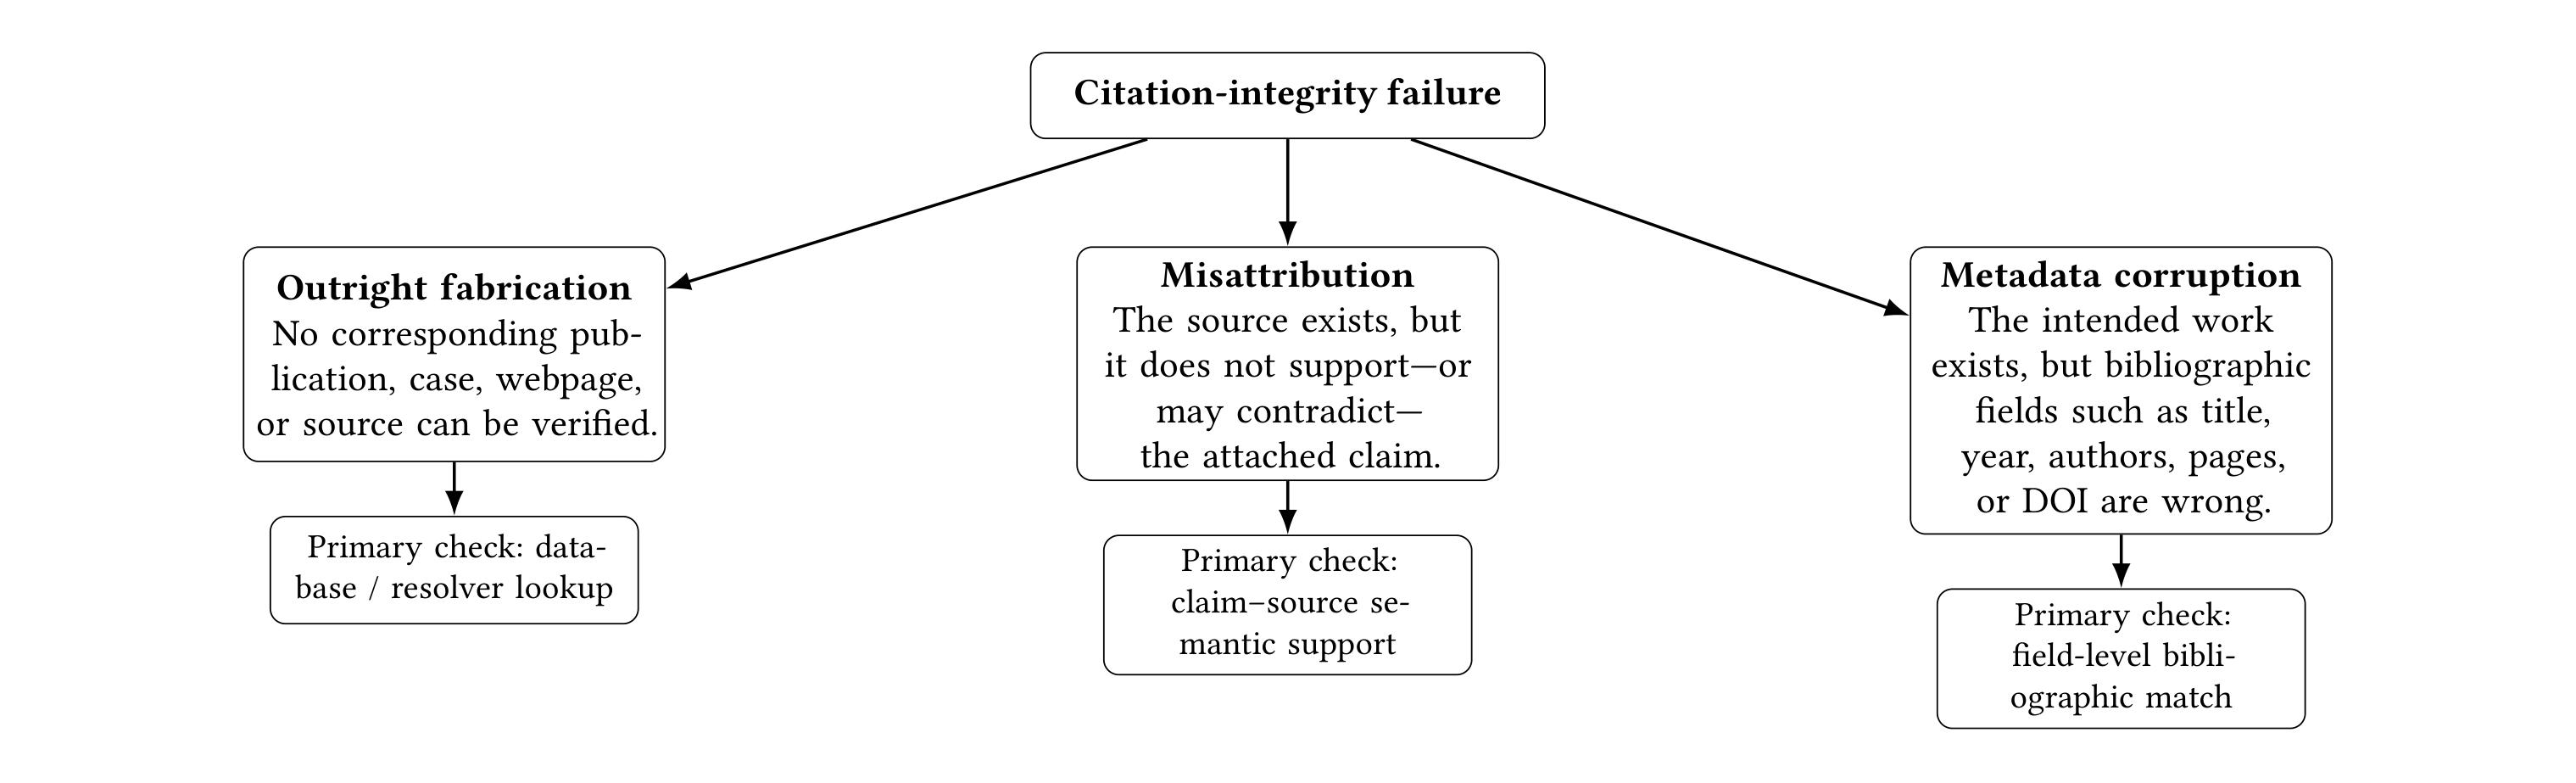
\includegraphics[width=\linewidth]{figures/figure1.png}\caption{1. Taxonomy of citation-integrity failure modes used in this review. A single generated bibliography may contain all three classes, but each class requires a different verification action.}\end{figure}
\subsection{Agentic Search and Verifiability}

A clickable citation provides a beginning for the reader. Liu et al. posed the question about the material they were linked to. Supported the sentence and if the sentence needed evidence there were sufficient cita- tions \cite{ref13}. An examination of news attribution looks at related concerns in non-scholarly publications. \cite{ref10}. Of course, the input to search answers is the passage and the claim, with useful evidence being the former. more than a mere connection.

\section{Taxonomy and Measurement Framework}

\subsection{Three Citation-Integrity Failure Modes}

Fabrication: Have you seen a work which you cite? Prior to determining that an entry is fabricated, the auditor needs a documented search procedure, where misspelled title and metadata is allowed. If no match is found after perusing one index, the case is left unresolved, but without entering into the other \cite{ref22}. Corruption of metadata: once identified, you can correct the work’s authors, title, year and all of this metadata. Is the record of fields matching the publication record? A real paper containing a false year should go in here \cite{ref2,ref17}. Misattribution: Is the identifiable source of the particular statement capable of supporting the statement? A paper may Have a conversation with each other, but not to support the reported outcome \cite{ref13,ref23} Metadata errors and misattribution is possible within an entry.

\subsection{Core Reporting Metrics}

A simple fabrication rate (SFR) can be reported as
\begin{equation}\mathrm{FR}=\frac{N_{\mathrm{fabricated}}}{N_{\mathrm{citations}}}\times100\%,\end{equation}
Where citations are listed in the numerator, it should only be cited as nonexistent on a study where that is the result of a study verification. rule. Unless the reader of equation (1) would expect a metadata error or unsupported claim to be included silently, Equation (1) should not contain such a metadata error or unsupported claim. Those cases are specifically set out as “fabrication” in the paper itself. Therefore, a complementary support rate is given for systems that add citations to the generated claims.
\begin{equation}\mathrm{SR}=\frac{N_{\text{supported claim-citation pairs}}}{N_{\text{evaluated claim-citation pairs}}}\times100\%.\end{equation}
\begin{table}[htbp]\caption{Representative empirical evidence on citation fabrication and citation support. Rates follow each source study’s own definition and are not directly interchangeable.}\centering\footnotesize\setlength{\tabcolsep}{2pt}\begin{tabular}{@{}p{.18\linewidth}p{.24\linewidth}p{.28\linewidth}p{.25\linewidth}@{}}\toprule
Study & System / setting & Reported result & Comparison caveat \\
Walters \& Wilder \cite{ref22} & GPT-3.5, GPT-4; multidisciplinary reviews & 55\% fabricated (GPT-3.5), 18\% (GPT-4); errors remained in real citations & Closed-book, version- and prompt-specific \\
Magesh et al. \cite{ref14} & Commercial legal RAG systems & 17–33\% hallucination in the tools evaluated & Proprietary retrieval/ranking not observable \\
Liu et al. \cite{ref13} & Generative web search engines & 51.5\% of sentences fully supported; 74.5\% citation correctness & Measures claim support, not source existence alone \\
Wu et al. \cite{ref23} & Medical LLM answers, including search-enabled systems & Many responses not fully supported despite valid URLs & Domain-specific automated and expert evaluation \\
Linardon et al. \cite{ref12} & GPT-4o mental-health literature reviews & 35/176 fabricated; rates differed across the three topics & Six prompts and one model family \\
Naser \cite{ref18} & Ten commercial LLMs, four academic domains & 11.4–56.8\% hallucination across 69,557 citations & Large preprint audit; still protocol-dependent \\\bottomrule\end{tabular}\end{table}
The measure, equation (2), is actually a semantic attribution measure, not a measure of the existence of the source. Together, Eqs. (1) and (2) avoid having one headline number combine multiple layers of citation integrity.

\section{Comparative Synthesis of Empirical Evidence}

Table 1 summarizes representative empirical studies. The table intentionally preserves the original study definitions rather than converting all results into one artificial common metric.

\subsection{Model Generation and Capability Scaling}

Under the prompts used by Walters and Wilder, the proportion of fabricated references was lower for GPT-4 than for GPT-3.5 \cite{ref22}. That comparison holds the task relatively steady. Comparing a percentage from one study with a percentage from a different prompt set cannot isolate the effect of model generation. The cross-model audit in Table 1 should likewise be interpreted within its own protocol \cite{ref18}.

\subsection{Retrieval Helps, not Solves, Citation Failure}

Either selected retrieval provides material to quote, or retrieved material may be incorrect or not necessary, or the passage may be irrelevant to the question posed. The answer the student might produce might be more extensive than this. Research into legal tools and also outputs in the RAGTrueh corpus. errors of retrieval are illustrated in a retrieval setting \cite{ref14,ref19}. In order to distinguish retrieval failure from If a writing error has been made, the auditor will require the retrieved passages and final answer. A The proprietary interface may only be used for the latter.

\subsection{All the evidence is not created equal.Not all citations are created equal.}

For the generative-search audit, 51.5\% of the sentences generated were supported entirely by citations. The average score for these citations was 74.5\%, which was higher than the average scores for associated sentences \cite{ref13}. The first percentage There are two counters: one for sentences, one for citations. There is no way to determine the number of publications that were not. invented.
\begin{figure}[htbp]\centering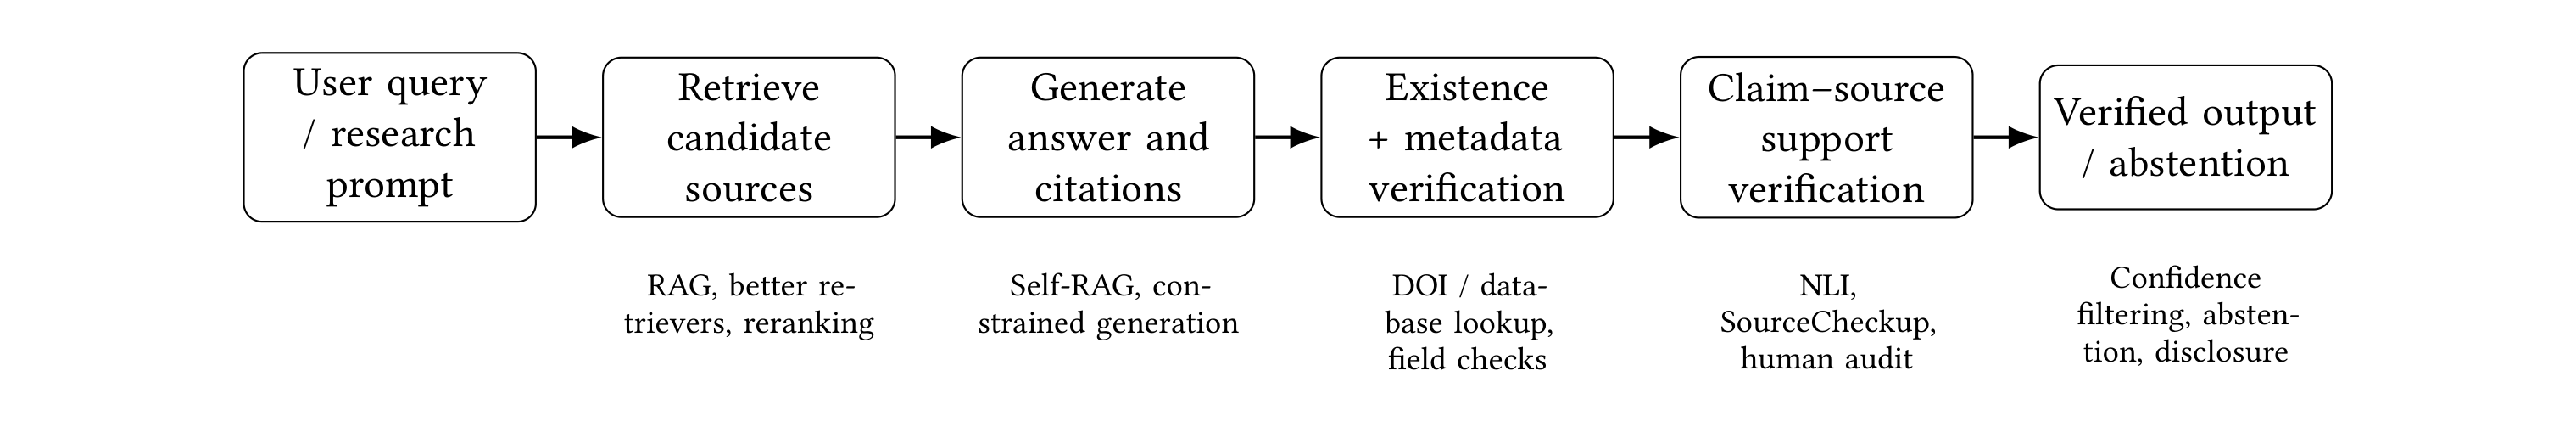
\includegraphics[width=\linewidth]{figures/figure2.png}\caption{2. End-to-end citation-verification pipeline. Controls for Retrieval, Generation and Biblio- graphic validation, disclosure/sentinement support checking, and final disclosure or abstention.}\end{figure}
\begin{table}[htbp]\caption{Representative methods of prevention, detection and auditing.}\centering\footnotesize\setlength{\tabcolsep}{2pt}\begin{tabular}{@{}p{.36\linewidth}p{.61\linewidth}@{}}\toprule
\multicolumn{2}{p{.96\linewidth}}{Target Strength and residual limitation are addressed by approaching them.Strength of primary target and residual limitation can be approached.} \\ \midrule
RAG \cite{ref14,ref19} & Even though the tape is retrieved, its content is not returned to the RAG.The RAG remains “offline” when the tape is retrieved. evidence Practical and effective – but perhaps poor retrieval or unsupported However, even with synthesis, it always gives false citations. \\
- Self-RAG \cite{ref1} & Retrieval + self-critique; relies on learned reflection quality \\
SelfCheckGPT \cite{ref15} & Sampling-inconsistency Black-box and zero-resource; consistent errors can still appear reliable \\
Sentence entropy: & More robust than surface agreement; requires multiple semantic interpretations \cite{ref7} Gedanken-years of research have gone into developing this measure. generations Avoids the indirect testing of attribution required by SourceCheckup \cite{ref23} (Claim–source support); domain calibration and Despite automated judging, some geographical restrictions still exist. \\
ALCE / LegalCiteBench \cite{ref5,ref8} & Citation of sources and reli- ability Applying a reusable approach to evaluation consisting of citations and/or scores; distributions remain task-specific \\\bottomrule\end{tabular}\end{table}
Medical source checking may be yet another situation in which valid links do not support. For every answer, include each statement in the answers \cite{ref23}.

\section{Current Approaches to Detection, Mitigation, and Benchmarking}

The main intervention points on retrieval to final verification were plotted on the diagram shown in Figure 2. Table 2 then compares Suggest representative approaches according to the target, strength and residual limitations.

\subsection{Retrieval Grounding and Self-Reflective Generation.}

Include Where a case has occurred where an answer has been generated that has not been backed up by RAGTruth, it is documented. retrieved material \cite{ref19}. Self-RAG adds retrieval decisions and reflection to generation \cite{ref1}. RAGChecker offers diagnostics for the components of retrieval and generation \cite{ref21}. For a given error, The first functional difference has to do with whether or not the passage necessary was retrieved. If it was, the next The question at hand is what kind of use was made of this answer. Discover how to benchmark Citation Fabrication Across Large Language

Models (LLMs) and agentic search tools.Understand how to evaluate LLMs and agentic search tools’ capabilities and behaviours with regards to Citation Fabrication.

\subsection{Consistency-Based Detection}

In the case of SelfCheckGPT, the flag is raised when there are differences in samples \cite{ref15}. Semantic entropy accounts One technical challenge is that a number of different answers may be intended to convey the same message (for example, "valving" vs "housed in a valve"). For citation Variation may be useful in prioritising records to be audited. Unagreement will not resolve the issue of whether the The same incorrect title appears more than once: cited item exists

\subsection{Claim-Level and Atomic-Fact Verification}

FActScore breaks an answer into atomic factual statements and checks them against a knowledge source \cite{ref16}. SourceCheckup assesses associations between a medical statement and the cited information \cite{ref23}. When a source provides support for the first clause and the second clause is of similar length, splitting the sentence can be very helpful. The second is not mentioned anything. Whoever, being of memory lax, remembers not the step of his foot, shall deny that he has taken it.He who is scant of memory and forgets the steps in his foot will say that he did not take them. inspectable.

\subsection{Citation-Specific Benchmarks}

For a cited-answer task, ALCE assesses fluency, the correctness of the answers, the quality of the citations \cite{ref8}. Legal- CiteBench is dedicated to tasks of legal citation \cite{ref5}, while HALoGEN tests hallucination in terms of domains \cite{ref20}. Bolden pinpoints the type of inequality for which the choice of benchmark arises: a reference string, a Someone has the legal right, or they make a claim, in a generated solution.

\section{Research Challenges and Limitations of Existing Evidence}

The current limitations and challenges of the available evidence are summarized below.Seven challenges and limitations of the available evidence are summarized below.

\subsection{Inconsistent Operational Definitions}

If the study includes one "false" DOI and the next one is correct, the figure for the "false" rate will be different based on the first study than the second. sets the identity of the paper to be intended. A coding guide can be shipped that provides examples of both actual 6 Gorla Nitheesh Kumar and the opposite they’re fake. Process a title with a faulty DOI with no resolved title. It should also indicate whether re-entry is allowed or not Only once every incidence or event.

\subsection{Prompt/Protocol Sensitivity (2 points)}

The request itself influences the type of citations which will be included within the sampling, if there are any. A system asked for Less than 10 papers may be returned or may not be returned at all. Given a number, report its report number. returned and the number that could be adjudicated. Keep prompt and the visible system unchanged. These are the other counts that are patiented with in collaboration with \cite{ref12,ref18}.

\subsection{Rapid Model Turnover And Benchmark Decay}

Not all of the components of a search system can be identified with a product label. A difference between The two runs could be due to Kansas City’s normal range in response or to an index change or system update. Dated cluster recurrences from between-window signals or trends.Rejections

and reruns in a same collection window can be used to separate the within-window rejections from between-window signals or trends. They don’t identify the cause of change but rather the variation from a subsequent change.

\subsection{Restricted Auditability of Proprietary Systems.}

7.4 Purpose: To provide limited audibility of proprietary systems. If a tool provides an answer and a link but not retrieval trace, then the auditor may look at the answer. opposing the source that was linked in. In most instances, it is impossible for the auditor to determine if a better source was ever, Was not retrieved, was ranked below its rank or ignored when generated. The observed failure and its Anything that is considered as being a possible cause should be mentioned separately.

\subsection{Domain and Language Coverage}

The term “scholarly writing” is applied to the English-language scholarly work; in addition, the studies reviewed include medicine, US law, and web. search. Within specific protocols, variations across topics and disciplines have been found \cite{ref12,ref17}. If the collection is not well-indexed, the failure of the index to find a work can testify as strongly as anything to the value of the index. about the model. Such environments require a method of keeping unexplored records.

\section{Research Gaps and Future Directions}

The gaps below follow from comparative evidence and methodological shortcomings. identified in Section 7.

\subsection{A Standardized Multi-Layer Citation Benchmark.}

One possible measure would be to keep four judgements: that the source is there, that its source is reliable, that it has been fact-checked, and that it is balanced. The metadata is accurate, in support of the claim, and whether claims that require evidence have citations. There are different denominators for these judgments. Reporting them together would make Eqs. Neither (1) nor (2) can be reduced to a single score.

\subsection{Longitudinal, Versioned Evaluation}

Prior to comparing two dates, an audit should be done to determine the order of magnitude of the difference between the two dates if the same analysis is carried out. prompt is repeated in one collection period. Otherwise a difference was found that was considered to be caused by an update. might also occur between two runs on the same day. A helpfully released version would record the unedited For each run outputs, the time and a prompt, the text and visible mode.

\subsection{Scalable Misattribution Detection}

A passage-level verifier should determine which words in the source are supporting the claim and allow an insufficient-evidence decision. The testing of it against manually checked cases would reveal where The similarity of the topics is confused with support. Uncertain cases should be considered in the cost of the review. Together with classification performance, evaluation was performed.

\subsection{Evaluating cross-lingual and low-resource situations.}

The multilingual audit should be flexible enough to accommodate alternate spellings of author names, incom- full names for titles and titles that have been translated. plete index coverage. One practical test would be comparing the results of a single-index search to An adjudication that also
\begin{table}[htbp]\caption{Proposed minimum reporting standard for citation-integrity evaluations.}\centering\footnotesize\setlength{\tabcolsep}{2pt}\begin{tabular}{@{}p{.2\linewidth}p{.77\linewidth}@{}}\toprule
Item & Minimum information to report \\
System & Exact model/product name, version if available, date tested \\
Mode & Closed-book, web search, RAG, tools/agents enabled \\
Prompts & Full templates, citation instruction, number of turns \\
Sampling & Temperature, top-$p$, repetitions, deterministic settings \\
Dataset & Domain, language, query source, inclusion criteria \\
Labels & Explicit definitions of fabrication, metadata error, misattribution \\
Verification & Databases/resolvers used; claim-support annotation procedure \\
Metrics & Separate existence, metadata, support, and completeness measures \\
Reproducibility & Archived outputs, code, evaluator instructions, timestamps \\\bottomrule\end{tabular}\end{table}
employs regional indexes and publisher records. This would aid in differentiating this from others this way. A limitation on getting back to an invented reference.

\subsection{Human Factors and Interface Design}

A reader might also want to find out if a link is active, if the publication is pertinent, and if a particular passage supports the claim. Those judgments could be shown in a separate way in an interface. A user study would be required to assess if that display is effective at determining if an assertion is not supported. rather than simply increasing their confidence.

\subsection{A Reproducible Minimum Reporting Standard (MRS)}

Table 3 is a discussion of what another auditor must reconstruct to create an evaluation. Alongside the prompts The rules used to count and details of the system should be preserved in the audit, as should evidence of any matches that were unclear. Any reasons to exclude records.

\section{Conclusion}

A bibliography may include fewer bogus citations without providing readers with inadequate documentation of The assertions made in an answer. Researching the publication records shows that there are no records of publications and they are incorrect. fields. To check attribution, a separate observation is needed: the claim must be read against the background of the context in which it arose. cited passage. This is why the percentages gathered in Table 1 should not be thought of as interchangeable. measures of reliability. A next step is to duplicate an established scholarly request with documented conditions, for example: Discuss the difference in the number of fabrications measured by different responses. Such an audit should Keep unresolved cases, report citation yield and differentiate between metadata errors and missing publications. The results of its conclusions would be relevant to the prompts and set-up used. Establishing If all claims were to be substantiated, another level of audit would be required at the passage level.
\begin{thebibliography}{23}
\bibitem{ref1} Akari Asai, Zeqiu Wu, Yizhong Wang, Avirup Sil, and Hannaneh Hajishirzi. 2024. Self-RAG: Learning to Retrieve, Generate, and Critique through Self-Reflection. In The Twelfth International Conference on Learning Representations. https://openreview.net/forum?id=hSyW5go0v8

\bibitem{ref2} M. Bhattacharyya, V. M. Miller, D. Bhattacharyya, and L. E. Miller. 2023. High Rates of Fabricated and Inaccurate References in ChatGPT-Generated Medical Content. Cureus 15, 5 (2023), e39238.

\bibitem{ref3} Álvaro Cabezas-Clavijo and Pavel Sidorenko-Bautista. 2025. Assessing the Performance of 8 AI Chatbots in Bibliographic Reference Retrieval: Grok and DeepSeek Outperform ChatGPT, but None Are Fully Accurate. arXiv:2505.18059 [cs.IR]

\bibitem{ref4} Mohamed Chelli, Julien Descamps, Vincent Lavoué, Christophe Trojani, Mohamad Azar, Mathieu Deckert, Jean-Louis Raynier, Guillaume Clowez, Pascal Boileau, and Charlotte Ruetsch-Chelli. 2024. Hallucination Rates and Reference Accuracy of ChatGPT and Bard for Systematic Reviews: Comparative Analysis. Journal of Medical Internet Research 26 (2024), e53164. doi:10.2196/53164

\bibitem{ref5} Sijia Chen, Hang Yin, and Shunfan Zhou. 2026. LegalCiteBench: Evaluating Citation Reliability in Legal Language Models. arXiv:2605.10186 [cs.CL]

\bibitem{ref6} Matthew Dahl, Varun Magesh, Mirac Suzgun, and Daniel E. Ho. 2024. Large Legal Fictions: Profiling Legal Hallucinations in Large Language Models. Journal of Legal Analysis 16, 1 (2024), 64–93. doi:10.1093/jla/laae003

\bibitem{ref7} Sebastian Farquhar, Jannik Kossen, Lorenz Kuhn, and Yarin Gal. 2024. Detecting Hallucinations in Large Language Models Using Semantic Entropy. Nature 630, 8017 (2024), 625–630. doi:10.1038/s41586-024-07421-0

\bibitem{ref8} Tianyu Gao, Howard Yen, Jiatong Yu, and Danqi Chen. 2023. Enabling Large Language Models to Generate Text with Citations. In Proceedings of the 2023 Conference on Empirical Methods in Natural Language Processing. 6465–6488. doi:10.18653/v1/2023.emnlp-main.398

\bibitem{ref9} Lei Huang, Weijiang Yu, Weitao Ma, Weihong Zhong, Zhangyin Feng, Haotian Wang, Qianglong Chen, Weihua Peng, Xiaocheng Feng, Bing Qin, and Ting Liu. 2025. A Survey on Hallucination in Large Language Models: Principles, Taxonomy, Challenges, and Open Questions. ACM Transactions on Information Systems 43, 2 (2025), 1–55. doi:10.1145/3703155

\bibitem{ref10} Klaudia Jazwinska and Aakanksha Chandrasekar. 2025. AI Search Has a Citation Problem. Columbia Journalism Review, Tow Center for Digital Journalism. https://www.cjr.org/tow\_center/we-compared-eight-ai-search-engines-theyre-all-bad-at-citing-news.php

\bibitem{ref11} Ziwei Ji, Nayeon Lee, Rita Frieske, Tiezheng Yu, Dan Su, Yan Xu, Etsuko Ishii, Ye Jin Bang, Andrea Madotto, and Pascale Fung. 2023. Survey of Hallucination in Natural Language Generation. Comput. Surveys 55, 12, Article 248 (2023). doi:10.1145/3571730

\bibitem{ref12} Jake Linardon, Hannah K. Jarman, Zoe McClure, Cleo Anderson, Claudia Liu, and Mariel Messer. 2025. Influence of Topic Familiarity and Prompt Specificity on Citation Fabrication in Mental Health Research Using Large Language Models: Experimental Study. JMIR Mental Health 12 (2025), e80371. doi:10.2196/80371

\bibitem{ref13} Nelson F. Liu, Tianyi Zhang, and Percy Liang. 2023. Evaluating Verifiability in Generative Search Engines. In Findings of the Association for Computational Linguistics: EMNLP 2023. 7001–7025. doi:10.18653/v1/2023.findings-emnlp.467

\bibitem{ref14} Varun Magesh, Faiz Surani, Matthew Dahl, Mirac Suzgun, Christopher D. Manning, and Daniel E. Ho. 2025. Hallucination-Free? Assessing the Reliability of Leading AI Legal Research Tools. Journal of Empirical Legal Studies 22, 2 (2025), 216–242. doi:10.1111/jels.12413

\bibitem{ref15} Potsawee Manakul, Adian Liusie, and Mark J. F. Gales. 2023. SelfCheckGPT: Zero-Resource Black-Box Hallucination Detection for Generative Large Language Models. In Proceedings of the 2023 Conference on Empirical Methods in Natural Language Processing. 9004–9017. doi:10.18653/v1/2023.emnlp-main.557

\bibitem{ref16} Sewon Min, Kalpesh Krishna, Xinxi Lyu, Mike Lewis, Wen tau Yih, Pang Wei Koh, Mohit Iyyer, Luke Zettlemoyer, and Hannaneh Hajishirzi. 2023. FActScore: Fine-Grained Atomic Evaluation of Factual Precision in Long Form Text Generation. In Proceedings of the 2023 Conference on Empirical Methods in Natural Language Processing. 12076–12100.

\bibitem{ref17} Joshua Mugaanyi, Liang Cai, Shuo Cheng, Chao Lu, and Jun Huang. 2024. Evaluation of Large Language Model Performance and Reliability for Citations and References in Scholarly Writing: Cross-Disciplinary Study. Journal of Medical Internet Research 26 (2024), e52935. doi:10.2196/52935

\bibitem{ref18} M. Z. Naser. 2026. How LLMs Cite and Why It Matters: A Cross-Model Audit of Reference Fabrication in AI-Assisted Academic Writing and Methods to Detect Phantom Citations. arXiv:2603.03299 [cs.CL]

\bibitem{ref19} Cheng Niu, Yuanhao Wu, Juno Zhu, Siliang Xu, KaShun Shum, Randy Zhong, Juntong Song, and Tong Zhang. 2024. RAGTruth: A Hallucination Corpus for Developing Trustworthy Retrieval-Augmented Language Models. In Proceedings of the 62nd Annual Meeting of the Association for Computational Linguistics. 10862–10878. doi:10.18653/v1/2024.acl-long.585

\bibitem{ref20} Abhilasha Ravichander, Shubham Ghela, David Wadden, and Yejin Choi. 2025. HALoGEN: Fantastic LLM Hallucinations and Where to Find Them. In Proceedings of the 63rd Annual Meeting of the Association for Computational Linguistics. 1402–1425.

\bibitem{ref21} Dongyu Ru, Lin Qiu, Xiangkun Hu, Tianhang Zhang, Peng Shi, Shuaichen Chang, Cheng Ji, Chuan Wang, Shichao Sun, Huajian Li, Zeyu Zhang, Bin Wang, Jun Jiang, Tao He, Zhizheng Wang, Pengfei Liu, Yue Zhang, and Zheng Zhang. 2024. RAGChecker: A Fine-Grained Framework for Diagnosing Retrieval-Augmented Generation. In Advances in Neural Information Processing Systems, Vol. 37.

\bibitem{ref22} William H. Walters and Esther Isabelle Wilder. 2023. Fabrication and Errors in the Bibliographic Citations Generated by ChatGPT. Scientific Reports 13, Article 14045 (2023). doi:10.1038/s41598-023-41032-5

\bibitem{ref23} Kevin Wu, Eric Wu, Kevin Wei, Angela Zhang, Allison Casasola, Teresa Nguyen, Sith Riantawan, Patricia Shi, Daniel Ho, and James Zou. 2025. An Automated Framework for Assessing How Well LLMs Cite Relevant Medical References. Nature Communications 16, Article 3615 (2025). doi:10.1038/s41467-025-58551-6
\end{thebibliography}\end{document}